% ----------------------------------------------------------------------------------------
% 	Section Data Preparation
% ----------------------------------------------------------------------------------------
\section{Data Preparation}
\begin{frame}
    \sectionpage
\end{frame}

\begin{frame}
    \frametitle{Processing Genotype Data}

    \begin{enumerate}
        \item Hierarchical clustering by complete distance.

        We got $949$ blocks where the SNPs within a block differed by at most $1$ sample. 

        \item Select representative SNPs. 
        
        For each block, we choose a representative SNP with the most repetitions. 

        \item[$\blacksquare$] Marginal gene-marker association analysis. 
        
        Discussed in the following. 
    \end{enumerate}
\end{frame}

\begin{frame}
    \frametitle{Processing Expression Level Data}

    We choose genes according to MAPK signaling pathways \footnote[2]{Kanehisa, M., Goto, S., Sato, Y., Kawashima, M., Furumichi, M. and Tanabe, M. (2014) Data, information, knowledge and principle: Back to metabolism in KEGG. Nucleic Acids Res., 42, D199–D205.}

    \begin{figure}[h]
        \centering
        \includegraphics[width=0.75\textwidth]{./figs/MAPK.png}
    \end{figure}
\end{frame}

\begin{frame}\frametitle{Easy-to-use Data}
    Let $X$ represent the SNPs matrix, $Y$ represent the gene expression levels matrix, we obtain
    \begin{equation*}
        X\in\mathbb{R}^{949\times112} \quad,\quad Y\in\mathbb{R}^{53\times112}
    \end{equation*}

    Hereinafter, we denote $p$ as the number of explanatory variables, $q$ as the number of response variable, $n$ as the number of samples, $E$ as the random error matrix, and $B$ as the coefficient matrix, we can construct a multi-response linear model
    \begin{equation*}
        Y = XB + E. 
    \end{equation*}
    
\end{frame}



% ----------------------------------------------------------------------------------------
% 	Section Methodology
% ----------------------------------------------------------------------------------------
\section{Methodology}
\begin{frame}
    \sectionpage
\end{frame}

\begin{frame}
    \frametitle{Brief Introduction}

    \begin{itemize}
        \item Linear Regression Model
        \item Multi-response
        \item High Dimensional Problem
    \end{itemize}

\end{frame}

\begin{frame}
    \frametitle{Uni-Response Regression}

    Let $Y_j$ denote the $j$-th column of $Y$, represent the expression level of $j$-th gene. 

    An intuitive method is to regress each $Y_j$ with $X$, and we will get $q$ linear models. 
    We can use LASSO to get the estimated coefficient vector $\hat{\beta}_{(j)}\in\mathbb{R}^{p}$. 
    
    Then combine $q$ coefficient vectors $\hat{\beta}_{(j)}$ into a matrix $\widehat{B}\in\mathbb{R}^{p\times q}$ by column. 
\end{frame}

\begin{frame}
    \frametitle{Result of LASSO}

    \begin{figure}[h]
        \centering
        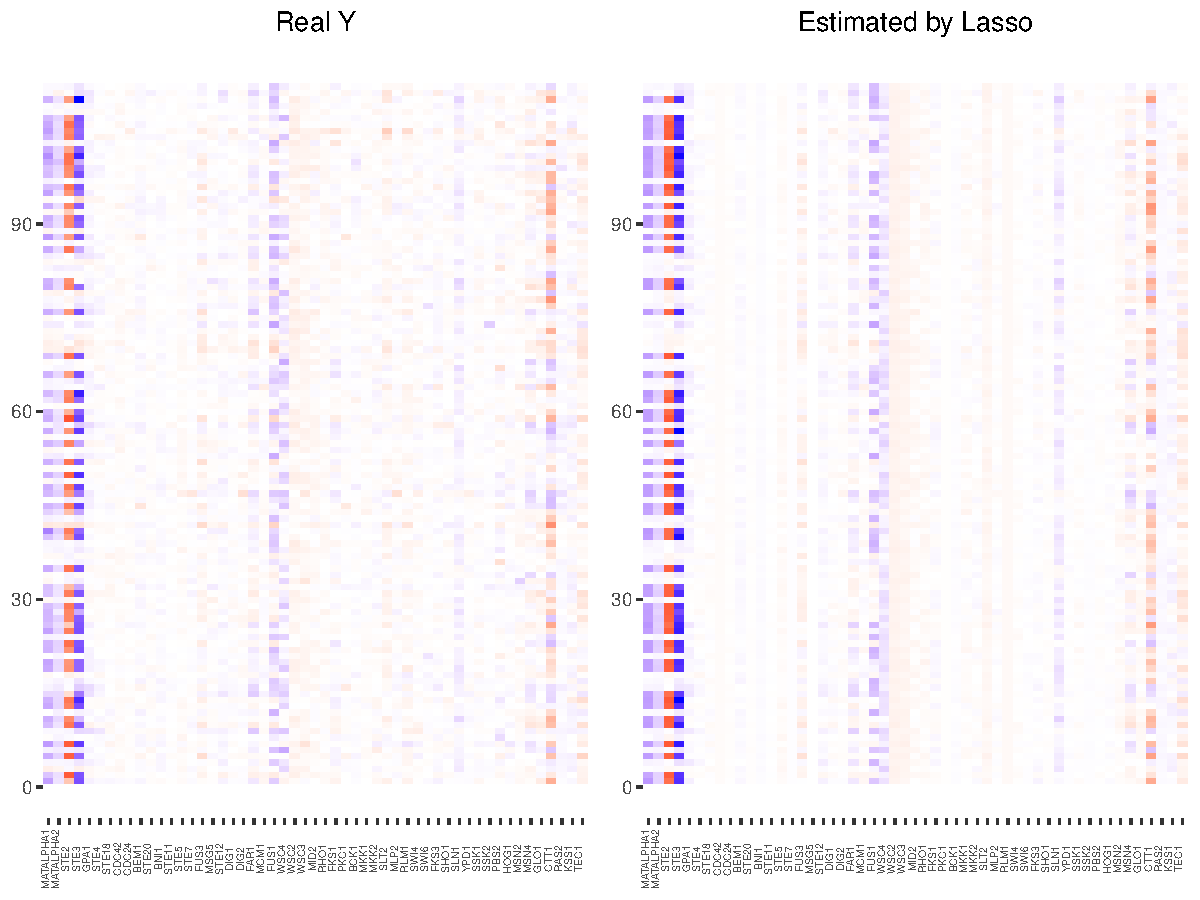
\includegraphics[width=0.8\textwidth]{./figs/heatmap_lasso.pdf}
        \caption{Heatmaps of real $Y$ and $\hat{Y}$ by LASSO}
    \end{figure}
\end{frame}

\begin{frame}
    \frametitle{Result of LASSO cont.}
    \begin{itemize}
        \item LASSO is a kind of shinkage estiamtion method. 
        So a sparse $\hat{\beta}_{(j)}$ is expected for each $j\in\{ 1,2,\dots,q \}$. 

        \item But $\widehat{B}$ may not be sparse by row. 
        
        Actually, there are $602$ nonzero rows in $\widehat{B}$ which has full column rank. 
    \end{itemize}
\end{frame}

\begin{frame}\frametitle{Group Sparse Linear Regression}
    Group sparse linear regression for multitask learning \footnote[1]{Dai, Ran, and Rina Foygel Barber. (2016)}
    \begin{equation}
        \widehat{B}=\underset{B}{\arg \min }\left\{\frac{1}{2}\|Y-X B\|_{F}^{2}+\lambda\|B\|_{(2,1)}\right\}
    \end{equation}
    where $\|\cdot\|_{F}$ is the Frobenius norm,% $\fronorm{M}=\sqrt{\sum_{ij}M_{ij}^2}$, 
    and where the $(2,1)$ norm in the penalty is given by
    $\|B\|_{(2,1)} = \sum_i \sqrt{\sum_j B_{ij}^2}$.

    This penalty promotes rowwise sparsity of $\widehat{B}$.
    % for large $\lambda$, $\widehat{B}$ will have many zero rows, however the nonzero rows will themselves be dense (no entrywise sparsity).
\end{frame}

\begin{frame}
    \frametitle{Result of GLasso}
    \begin{figure}[h]
        \centering
        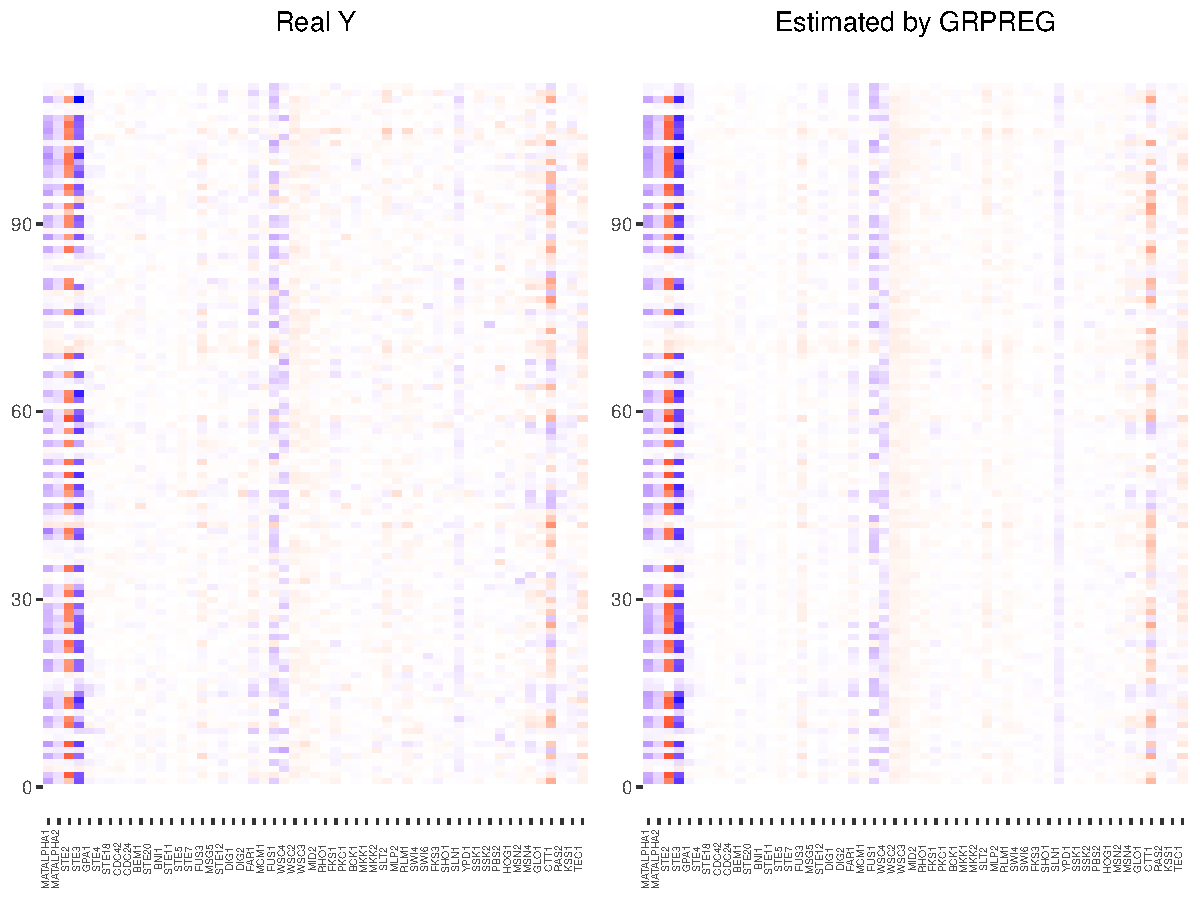
\includegraphics[width=0.8\textwidth]{./figs/heatmap_grpreg.pdf}
        \caption{Heatmaps. $\widehat{B}$ has full column rank and 201 non-zero rows.}
    \end{figure}
\end{frame}

\begin{frame}\frametitle{Biological Discovery}
    Previous biological research has revealed some facts which could be the guidelines for us to choose suitable method of data analysis.

    \begin{itemize}
%        \item analyze the influence of eQTLs(the quantitative trait loci) on the expression level of genes in the yeast MAPK signaling pathways. 
%        \item Biological characteristics of variables in the study(Gustin et al.(1998), and Brem and Kruglyak(2005)):
        
        \item Biological finding: 
        
              Each signaling pathway involves only a subset of genes\footnote[1]{Gustin, M. C., Albertyn, J., Alexander, M. and Davenport, K. (1998) Map kinase pathways in the yeast saccharomyces cerevisiae. Microbiology and Molecular Biology Reviews, 62, 1264–1300.}, which are regulated by only a few genetic variants.

        \item Corresponding characteristics in statistics: 
        
              The association structure between the eQTLs and the gene is of low rank and sparsity.
    \end{itemize}
\end{frame}

\begin{frame}{Multi-Response Regression}
    SOFAR \footnote[1]{Uematsu, Y., Fan, Y., Chen, K., Lv, J., \& Lin, W. (2019). SOFAR: large-scale association network learning. IEEE Transactions on Information Theory.} 
    uses the SVD decomposition $B= UDV^T$ and then impose penalties into $U$, $D$ and $V$ respectively. 
    \begin{equation}\footnotesize
        \begin{split}
            & (\widehat{D}, \widehat{U}, \widehat{V}) \\
            = & \underset{D, U, V}{\arg \min }\left\{\frac{1}{2} \left\|X- UDV^{T}\right\|_{F}^{2}+\lambda_{d}\|D\|_{1}+\lambda_{a} \rho_{a}(U D)+\lambda_{b} \rho_{b}(VD)\right\} \\ 
            & \quad\quad \text { subject to } U^{T} U=\mathbf{I}_{m}, \quad V^{T} V=\mathbf{I}_{m} 
        \end{split}
    \end{equation}
\end{frame}

\begin{frame}
    \frametitle{Result of SOFAR}
    \begin{figure}[h]
        \centering
        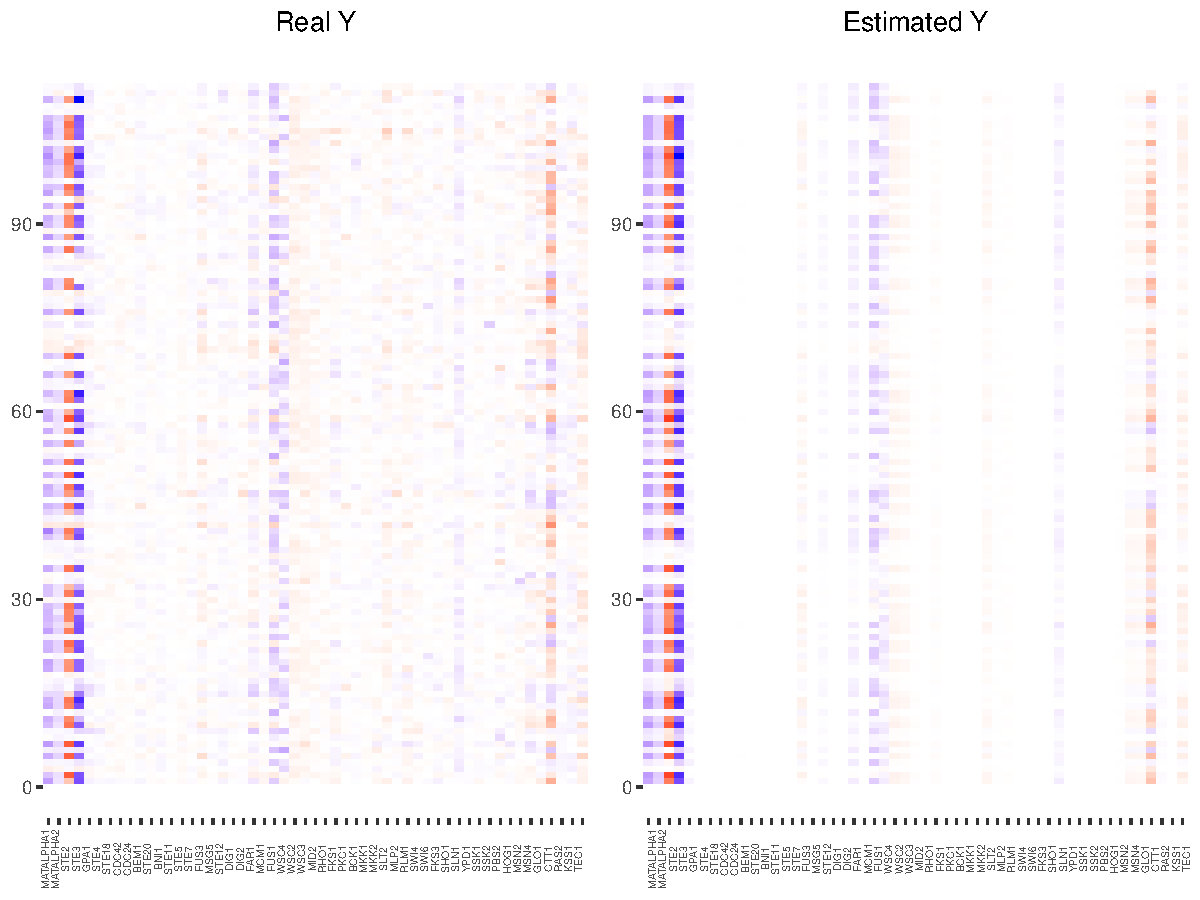
\includegraphics[width=0.8\textwidth]{./figs/heatmap1.pdf}
        \caption{Heatmaps of real $Y$ and $\hat{Y}$ by SOFAR}
    \end{figure}
\end{frame}

\begin{frame}
    \frametitle{Result of SOFAR cont.}
    \begin{figure}[h]
        \centering
        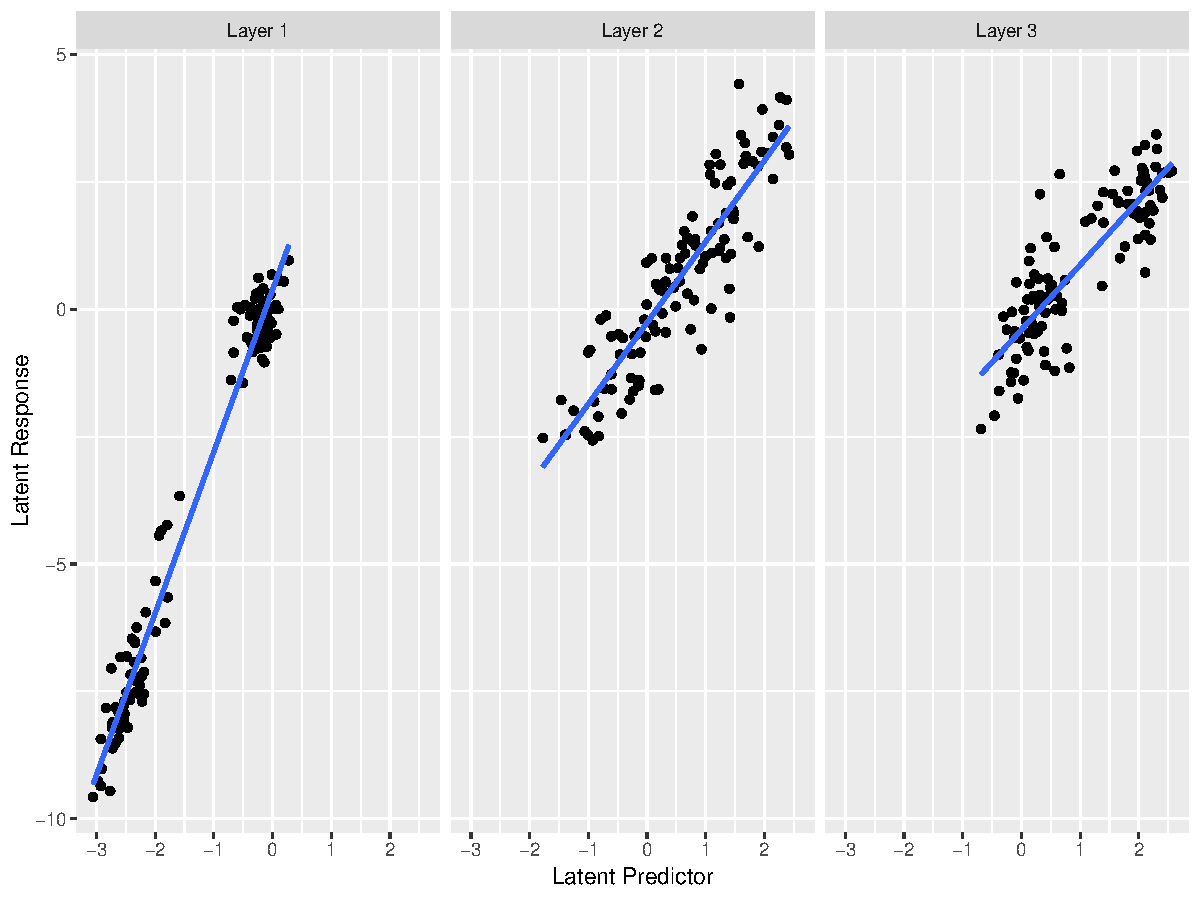
\includegraphics[width=0.75\textwidth]{./figs/latent1.pdf}
        \caption{Scatter plots of the latent responses versus the latent predictors in three SVD layers for the yeast data estimated by the SOFAR method}
    \end{figure}
\end{frame}


\begin{frame}
    \frametitle{Further Reduce Dimension of $X$}

    We performed a marginal gene-marker association analysis to identify SNPs that are associated with the expression levels of at least two genes with a p-value less than $0.05$, resulting in a total of $p = 776$ variables.

    Reduce additional $18.2\%$ $X$s. 

    Result: rank $3$ with $228$ non-zero rows in the estimation of $U$ and $25$ non-zero rows in the estimation of $V$. 
\end{frame}


\begin{frame}
    \frametitle{Result of SOFAR after Reduction}
    \begin{figure}[h]
        \centering
        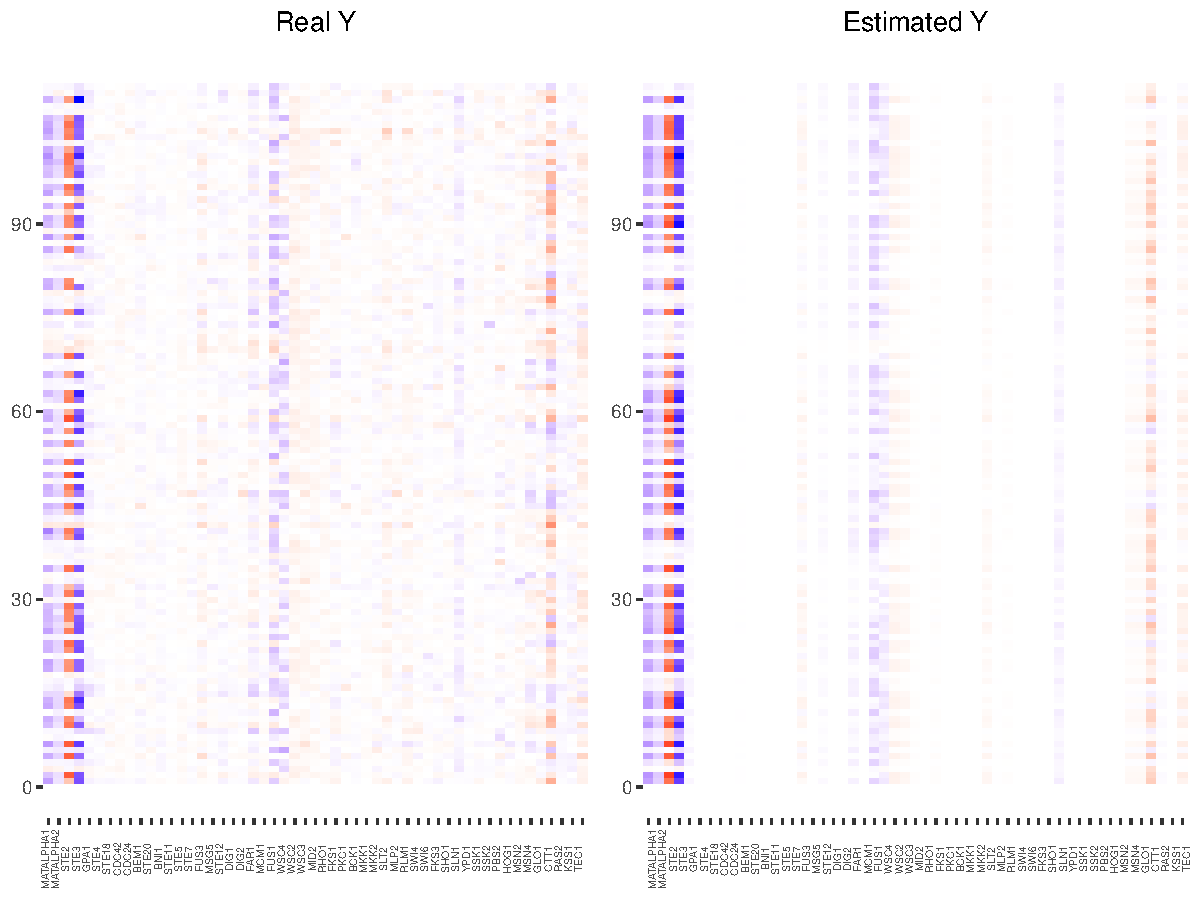
\includegraphics[width=0.8\textwidth]{./figs/heatmap2.pdf}
        \caption{Heatmaps of real $Y$ and $\hat{Y}$ by SOFAR}
    \end{figure}
\end{frame}

\begin{frame}
    \frametitle{Result of SOFAR after Reduction}
    \begin{figure}[h]
        \centering
        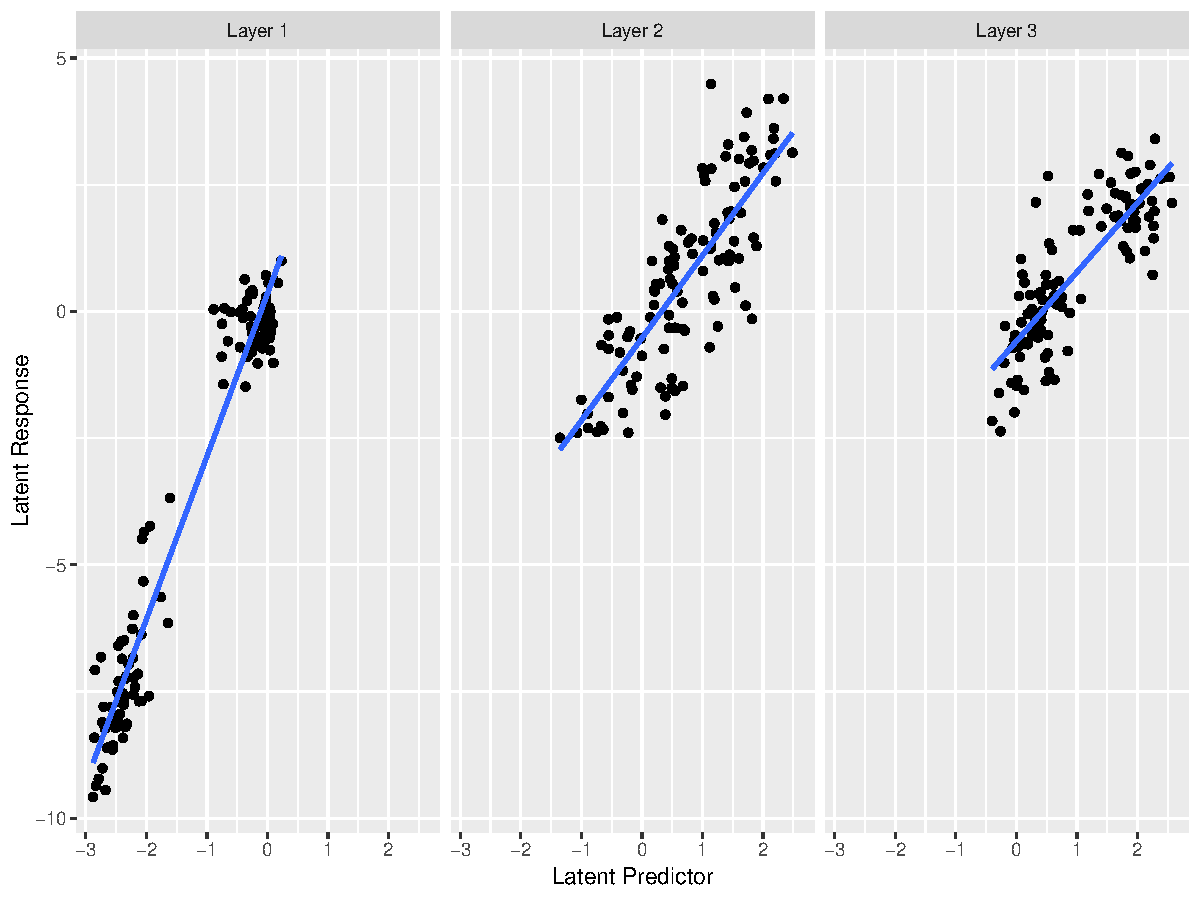
\includegraphics[width=0.75\textwidth]{./figs/letent2.pdf}
        \caption{Scatter plots of the latent responses versus the latent predictors in three SVD layers for the yeast data estimated by the SOFAR method}
    \end{figure}
\end{frame}

\begin{frame} \frametitle{$4$th Letent Pattern}
    \begin{figure}[h]
        \centering
        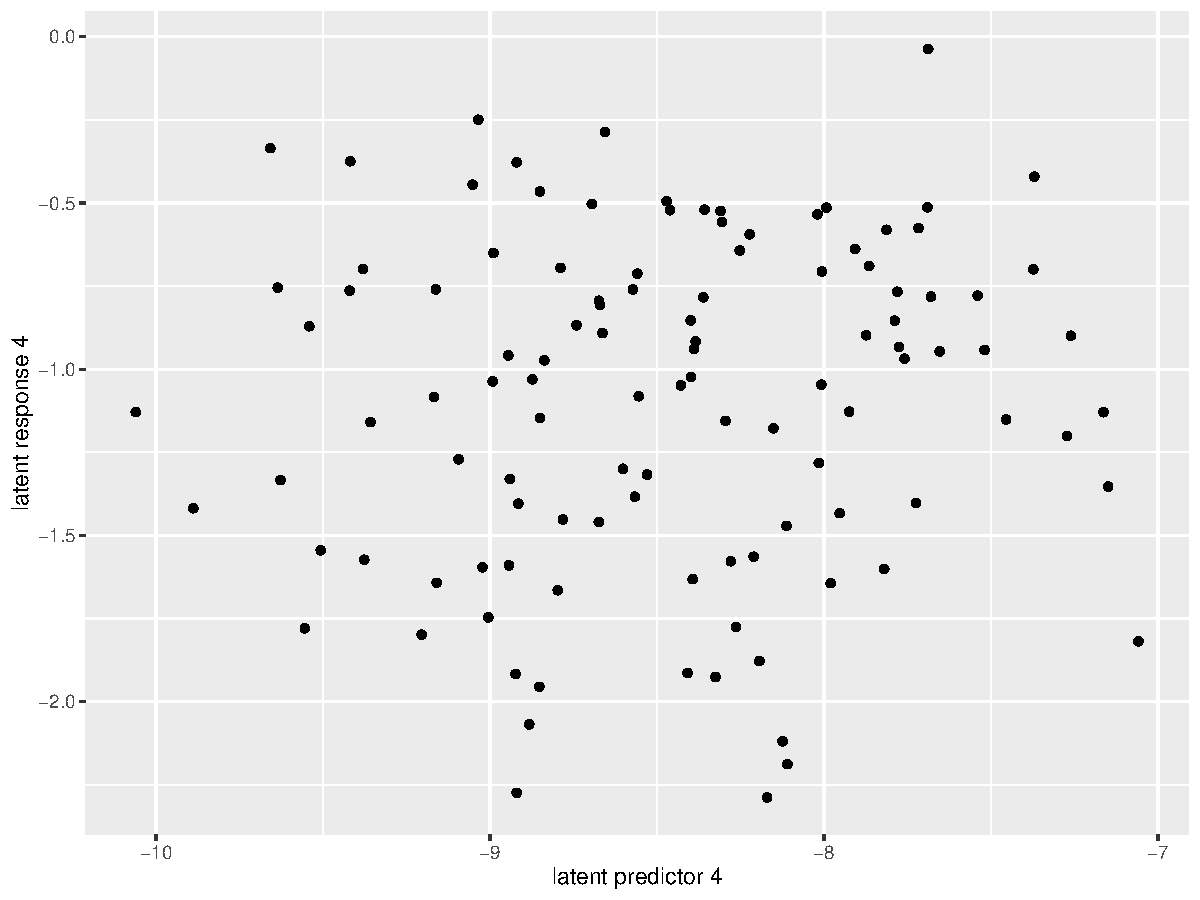
\includegraphics[width=0.75\textwidth]{./figs/latent4.pdf}
        \caption{Scatter plots of the $4$th latent responses versus the latent predictors for the yeast data estimated by the SOFAR method}
    \end{figure}
\end{frame}

